\documentclass{article}

\title{
  logit: Logistic Regression for Dichotomous
  Dependent Variables
}
\author{Matt Owen, Olivia Lau, Kosuke Imai, and Gary King}




\usepackage{bibentry}
\usepackage{graphicx}
\usepackage{natbib}
\usepackage{amsmath}
\usepackage{url}
\usepackage{Zelig}
\usepackage{Sweave}

%\VignetteIndexEntry{Logistic Regression for Dichotomous Dependent Variables}
%\VignetteDepends{Zelig, stats}
%\VignetteKeyWords{model,least squares,continuous, regression}
%\VignettePackage{Zelig}

\begin{document}

\nobibliography*



\section{Introduction}
\label{logit}

Logistic regression specifies a dichotomous dependent variable as a
function of a set of explanatory variables.

\section{Syntax}

\begin{verbatim}
> z.out <- zelig(Y ~ X1 + X2, model = "logit", data = mydata)
> x.out <- setx(z.out)
> s.out <- sim(z.out, x = x.out, x1 = NULL)
\end{verbatim}

\section{Additional Inputs} 

In addition to the standard inputs, {\tt zelig()} takes the following
additional options for logistic regression:  
\begin{itemize}
\item {\tt robust}: defaults to {\tt FALSE}.  If {\tt TRUE} is
selected, {\tt zelig()} computes robust standard errors via the {\tt
sandwich} package (see \cite{Zeileis04}).  The default type of robust
standard error is heteroskedastic and autocorrelation consistent (HAC),
and assumes that observations are ordered by time index.

In addition, {\tt robust} may be a list with the following options:  
\begin{itemize}
\item {\tt method}:  Choose from 
\begin{itemize}
\item {\tt "vcovHAC"}: (default if {\tt robust = TRUE}) HAC standard
errors. 
\item {\tt "kernHAC"}: HAC standard errors using the
weights given in \cite{Andrews91}. 
\item {\tt "weave"}: HAC standard errors using the
weights given in \cite{LumHea99}.  
\end{itemize}  
\item {\tt order.by}: defaults to {\tt NULL} (the observations are
chronologically ordered as in the original data).  Optionally, you may
specify a vector of weights (either as {\tt order.by = z}, where {\tt
z} exists outside the data frame; or as {\tt order.by = \~{}z}, where
{\tt z} is a variable in the data frame)  The observations are
chronologically ordered by the size of {\tt z}.
\item {\tt \dots}:  additional options passed to the functions 
specified in {\tt method}.   See the {\tt sandwich} library and
\cite{Zeileis04} for more options.   
\end{itemize}
\end{itemize}

\section{Examples}
\begin{enumerate}
\item {Basic Example}
 
Attaching the sample turnout dataset:
\begin{Schunk}
\begin{Sinput}
>  data(turnout)
\end{Sinput}
\end{Schunk}
Estimating parameter values for the logistic regression:
\begin{Schunk}
\begin{Sinput}
>  z.out1 <- zelig(vote ~ age + race,  model = "logit", data = turnout) 
> 
\end{Sinput}
\end{Schunk}
Setting values for the explanatory variables:
\begin{Schunk}
\begin{Sinput}
>  x.out1 <- setx(z.out1, age = 36, race = "white")
\end{Sinput}
\end{Schunk}
Simulating quantities of interest from the posterior distribution.
\begin{Schunk}
\begin{Sinput}
>  s.out1 <- sim(z.out1, x = x.out1)
\end{Sinput}
\end{Schunk}
\begin{Schunk}
\begin{Sinput}
>  summary(s.out1)
\end{Sinput}
\end{Schunk}
\begin{center}
\begin{Schunk}
\begin{Sinput}
>  plot(s.out1)
\end{Sinput}
\end{Schunk}
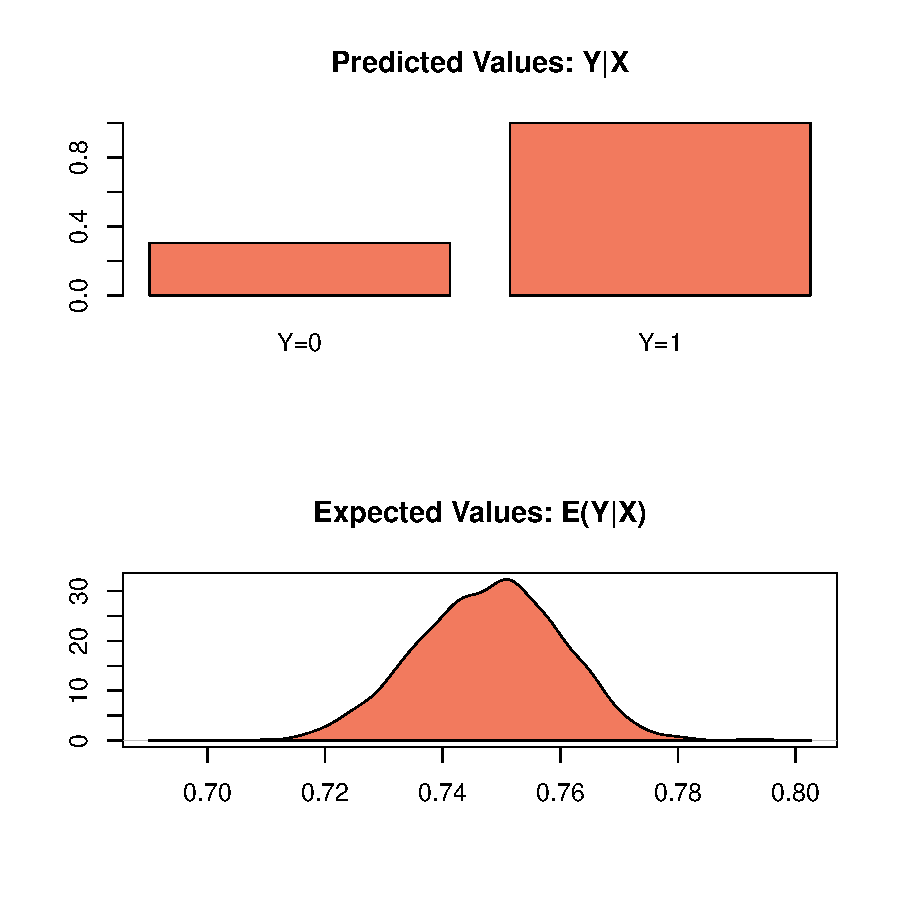
\includegraphics{logit-ExamplePlot}
\end{center}

\item {Simulating First Differences}

Estimating the risk difference (and risk ratio) between low education
(25th percentile) and high education (75th percentile) while all the
other variables held at their default values.
\begin{Schunk}
\begin{Sinput}
>  z.out2 <- zelig(vote ~ race + educate, model = "logit", data = turnout)
>  x.high <- setx(z.out2, educate = quantile(turnout$educate, prob = 0.75))
>  x.low <- setx(z.out2, educate = quantile(turnout$educate, prob = 0.25))
\end{Sinput}
\end{Schunk}

\begin{Schunk}
\begin{Sinput}
>  s.out2 <- sim(z.out2, x = x.high, x1 = x.low)
\end{Sinput}
\end{Schunk}
\begin{Schunk}
\begin{Sinput}
>  summary(s.out2)
\end{Sinput}
\end{Schunk}
\begin{center}
\begin{Schunk}
\begin{Sinput}
>  plot(s.out2)
\end{Sinput}
\end{Schunk}
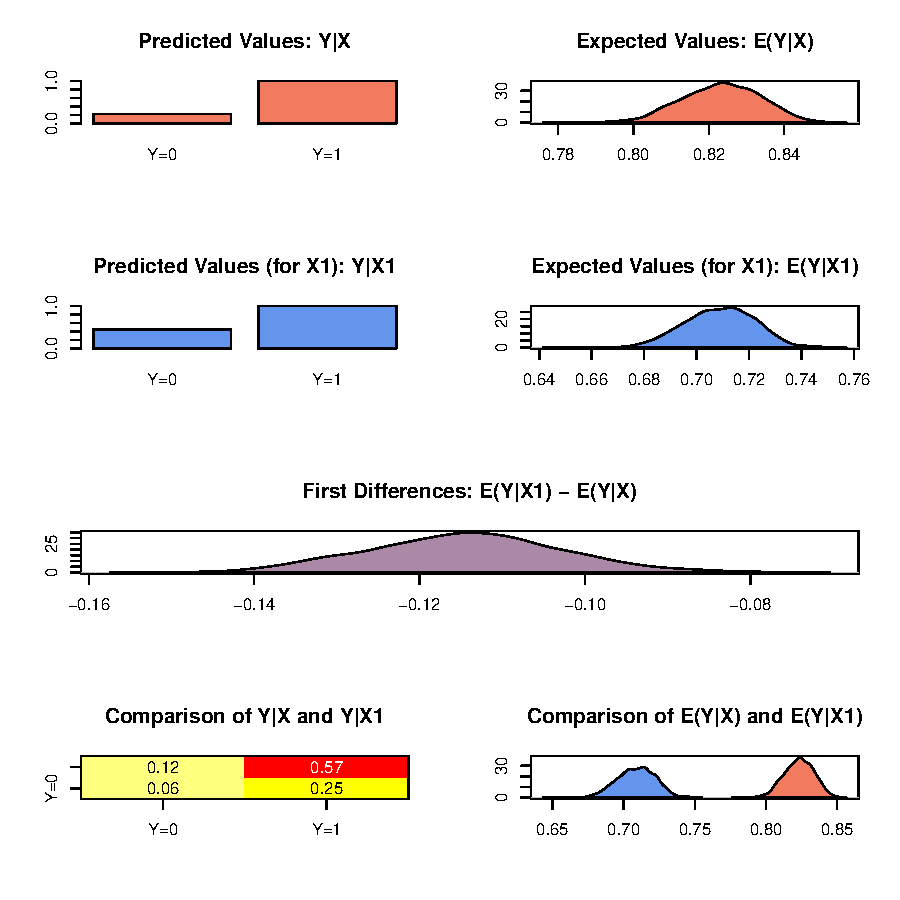
\includegraphics{logit-FirstDifferencesPlot}
\end{center} 


\item {Presenting Results: An ROC Plot}  \label{ROC}
  
  One can use an ROC plot to evaluate the fit of alternative model
  specifications.  (Use {\tt demo(roc)} to view this example, or see
  King and Zeng (2002)\nocite{KinZen02}.)  
\begin{Schunk}
\begin{Sinput}
>  z.out1 <- zelig(vote ~ race + educate + age, model = "logit", 
+                   data = turnout)
>  z.out2 <- zelig(vote ~ race + educate, model = "logit", data = turnout)
\end{Sinput}
\end{Schunk}
\begin{center}
\begin{Schunk}
\begin{Sinput}
> rocplot(z.out1$y, z.out2$y, fitted(z.out1), fitted(z.out2))
\end{Sinput}
\end{Schunk}
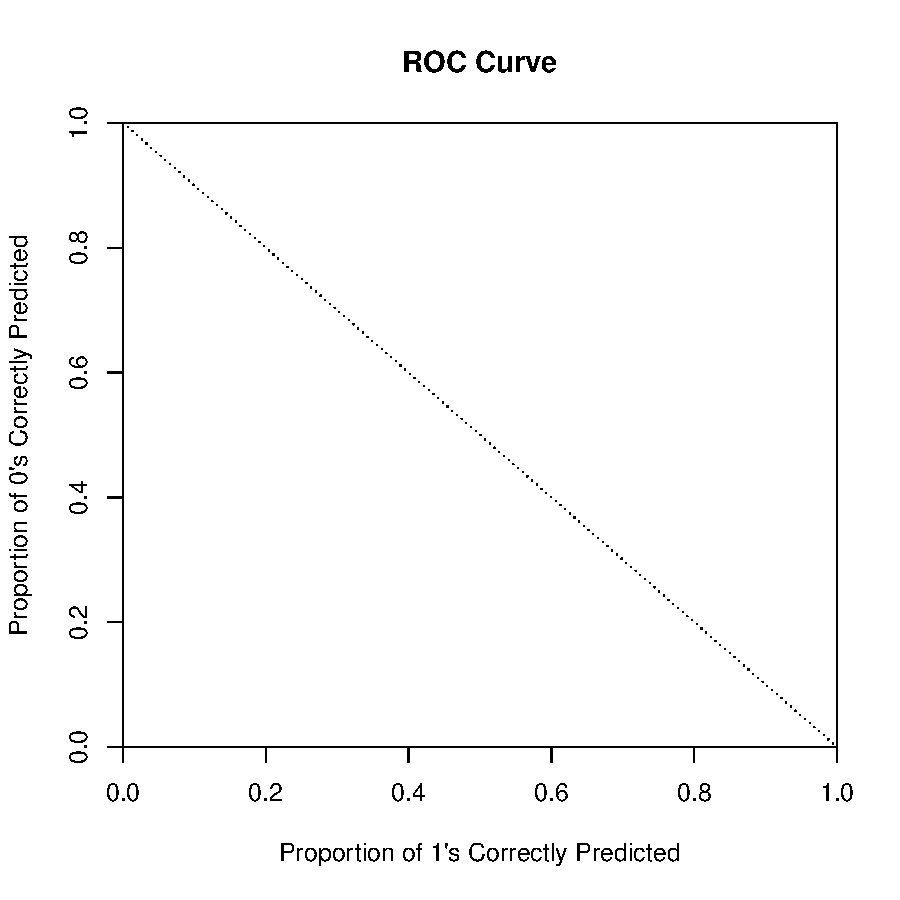
\includegraphics{logit-ROCPlot}
\end{center}
\end{enumerate}

\section{Model}
Let $Y_i$ be the binary dependent variable for observation $i$ which
takes the value of either 0 or 1.
\begin{itemize}

\item The \emph{stochastic component} is given by  
\begin{eqnarray*}
Y_i &\sim& \textrm{Bernoulli}(y_i \mid \pi_i) \\
    &=& \pi_i^{y_i} (1-\pi_i)^{1-y_i}
\end{eqnarray*}
where $\pi_i=\Pr(Y_i=1)$.

\item The \emph{systematic component} is given by: 
\begin{equation*}
\pi_i \; = \; \frac{1}{1 + \exp(-x_i \beta)}.
\end{equation*}
where $x_i$ is the vector of $k$ explanatory variables for observation $i$
and $\beta$ is the vector of coefficients.
\end{itemize}

\section{Quantities of Interest}
\begin{itemize}
\item The expected values ({\tt qi\$ev}) for the logit model are
  simulations of the predicted probability of a success: $$E(Y) =
  \pi_i= \frac{1}{1 + \exp(-x_i \beta)},$$ given draws of $\beta$ from
  its sampling distribution.

\item The predicted values ({\tt qi\$pr}) are draws from the Binomial
  distribution with mean equal to the simulated expected value $\pi_i$.  

\item The first difference ({\tt qi\$fd}) for the logit model is defined as
\begin{equation*}
\textrm{FD} = \Pr(Y = 1 \mid x_1) - \Pr(Y = 1 \mid x).
\end{equation*}

\item The risk ratio ({\tt qi\$rr}) is defined as
\begin{equation*}
\textrm{RR} = \Pr(Y = 1 \mid x_1) \ / \ \Pr(Y = 1 \mid x).
\end{equation*}

\item In conditional prediction models, the average expected treatment
  effect ({\tt att.ev}) for the treatment group is 
    \begin{equation*} \frac{1}{\sum_{i=1}^n t_i}\sum_{i:t_i=1}^n \left\{ Y_i(t_i=1) -
      E[Y_i(t_i=0)] \right\},
    \end{equation*} 
    where $t_i$ is a binary explanatory variable defining the treatment
    ($t_i=1$) and control ($t_i=0$) groups.  Variation in the
    simulations are due to uncertainty in simulating $E[Y_i(t_i=0)]$,
    the counterfactual expected value of $Y_i$ for observations in the
    treatment group, under the assumption that everything stays the
    same except that the treatment indicator is switched to $t_i=0$.

\item In conditional prediction models, the average predicted treatment
  effect ({\tt att.pr}) for the treatment group is 
    \begin{equation*} \frac{1}{\sum_{i=1}^n t_i}\sum_{i:t_i=1}^n \left\{ Y_i(t_i=1) -
      \widehat{Y_i(t_i=0)}\right\},
    \end{equation*} 
    where $t_i$ is a binary explanatory variable defining the
    treatment ($t_i=1$) and control ($t_i=0$) groups.  Variation in
    the simulations are due to uncertainty in simulating
    $\widehat{Y_i(t_i=0)}$, the counterfactual predicted value of
    $Y_i$ for observations in the treatment group, under the
    assumption that everything stays the same except that the
    treatment indicator is switched to $t_i=0$.
\end{itemize}

\section{Output Values}

The output of each Zelig command contains useful information which you
may view.  For example, if you run \texttt{z.out <- zelig(y \~\, x,
  model = "logit", data)}, then you may examine the available
information in \texttt{z.out} by using \texttt{names(z.out)},
see the {\tt coefficients} by using {\tt z.out\$coefficients}, and
a default summary of information through \texttt{summary(z.out)}.
Other elements available through the {\tt \$} operator are listed
below.

\begin{itemize}
\item From the {\tt zelig()} output object {\tt z.out}, you may
  extract:
   \begin{itemize}
   \item {\tt coefficients}: parameter estimates for the explanatory
     variables.
   \item {\tt residuals}: the working residuals in the final iteration
     of the IWLS fit.
   \item {\tt fitted.values}: the vector of fitted values for the
     systemic component, $\pi_i$.
   \item {\tt linear.predictors}: the vector of $x_{i}\beta$
   \item {\tt aic}: Akaike's Information Criterion (minus twice the
     maximized log-likelihood plus twice the number of coefficients).
   \item {\tt df.residual}: the residual degrees of freedom.
   \item {\tt df.null}: the residual degrees of freedom for the null
     model.
   \item {\tt data}: the name of the input data frame.  
   \end{itemize}

\item From {\tt summary(z.out)}, you may extract: 
   \begin{itemize}
   \item {\tt coefficients}: the parameter estimates with their
     associated standard errors, $p$-values, and $t$-statistics.
   \item{\tt cov.scaled}: a $k \times k$ matrix of scaled covariances.
   \item{\tt cov.unscaled}: a $k \times k$ matrix of unscaled
     covariances.  
   \end{itemize}

\item From the {\tt sim()} output object {\tt s.out}, you may extract
  quantities of interest arranged as matrices indexed by simulation
  $\times$ {\tt x}-observation (for more than one {\tt x}-observation).
  Available quantities are:

   \begin{itemize}
   \item {\tt qi\$ev}: the simulated expected probabilities for the
     specified values of {\tt x}.
   \item {\tt qi\$pr}: the simulated predicted values for the
     specified values of {\tt x}.
   \item {\tt qi\$fd}: the simulated first difference in the expected
     probabilities for the values specified in {\tt x} and {\tt x1}.
   \item {\tt qi\$rr}: the simulated risk ratio for the expected
     probabilities simulated from {\tt x} and {\tt x1}.
   \item {\tt qi\$att.ev}: the simulated average expected treatment
     effect for the treated from conditional prediction models.  
   \item {\tt qi\$att.pr}: the simulated average predicted treatment
     effect for the treated from conditional prediction models.  
   \end{itemize}
\end{itemize}






\subsection*{How to Cite the Logit Model}
\bibentry{ImaLauKin-logit11}

\subsection*{How to Cite the Zelig Software Package}
\CiteZelig


\subsection*{See also}
The logit model is part of the stats package by \citet{VenRip02}.
Advanced users may wish to refer to \texttt{help(glm)} and
\texttt{help(family)}, as well as \cite{McCNel89}. Robust standard
errors are implemented via the sandwich package by \citet{Zeileis04}.
Sample data are from \cite{KinTomWit00}.

\bibliographystyle{plain}
\bibliography{gk,gkpubs,Zelig}


\end{document}

%%% Local Variables: 
%%% mode: latex
%%% TeX-master: t
%%% End: 
